% This is mymiccaipaper.tex the demonstration file of
% MICCAI 2006 for Latex2e
% adapted from LLNCS.DEM from
% the LaTeX macro package from Springer-Verlag
% for Lecture Notes in Computer Science,
% version 2.2 for LaTeX2e
%
\documentclass{llncs}
%
\usepackage{makeidx}  % allows for indexgeneration
%

\usepackage{graphicx}
\graphicspath{{pics/}{figs/}}
% list here all the paths to your figure folders

\begin{document}
%
\frontmatter          % for the preliminaries
%
%\pagestyle{headings}  % switches on printing of running heads
\pagestyle{empty}  % switches off printing of running heads
%
\mainmatter              % start of your contributions
%
\title{Dynamic data analysis for pediatric airways}
%
\titlerunning{Short Title}  % abbreviated title (for running head)
%
\author{Chun-Wei Liu\inst{1}}
%
\authorrunning{C.-W. Liu}   % abbreviated author list (for running head)
%
%%%% modified list of authors for the TOC (add the affiliations)
\tocauthor{Chun-Wei Liu (University of North Carolina at Chapel Hill)}
%
\institute{Department of Computer Science,
University of North Carolina, Chapel Hill, \email{chunwei@cs.unc.edu}
}

% The following lines are used to remove authors and affiliations from
% the front page and running titles
\author{Chun-Wei Liu}
\authorrunning{C.-W. Liu}
\tocauthor{Chun-Wei Liu (UNC-CH)}
\institute{Department of Computer Science,\\
University of North Carolina, Chapel Hill, NC\\
\email{chunwei@cs.unc.edu}}

\maketitle              % typeset the title of the contribution

\begin{abstract}
The analysis of pediatric airway geometry using computed tomography (CT) images has provided rich diagnostic cues for doctors. Recently, dynamic CT data provides a better characterization of pediatric airways throughout the breathing cycle, for example to assess tracheomalacia. However, how to preprocess the increasing amount of dynamic data and how to analysis these data are still open questions. In this work, I performed dynamic data analysis using computer vision and machine learning approaches on synthetic and real airway data. In the future, I aim at building a 4D atlas for pediatric airways and to extend the approaches to other dynamic data modalities.
\end{abstract}

\section{Introduction}
\label{sec:intro}
% Why this problem is important?

% What 3D CT can do?
The analysis of pediatric airway geometry using 3D computed tomography (CT) images has provided rich cues for doctors to diagnose respiratory issue for patients.
Both radiologists and physicians have been working on the field for a while.
In image analysis side, radiologists Nakanoa et al. started to propose algorithm for measuring airway lumenal area using multidetector row CT~\cite{nakano2002development} one decade ago.
On the other hand, physicians continuously adopted benefits from imaging analysis for their clinical studies, for example, how well their patients with issues caused by airway were recovered after surgeries~\cite{abramson2011three}.
The progress made in image analysis these days was making the communication of both parties much easier by providing more informative statics from images.
For instance, given a CT image from a subject with some manually annotative landmarks, machine is able to learn from CT images of normal control data to build a subject-specific control atlas (a mean statics from the population of the subject.) 
Then machine can provide statics for where the positions have smaller cross-sectional area to doctors which makes diagnosing tracheal stenosis more actuary~\cite{hong2014statistical}.

% What 4D CT can do?
What can we learn from a four-dimensional CT (4D) image, an image set contains up to 16 3D CT images with respiratory motion induced image changes across the set that are not available on a single-component 3D CT image?
If an edge of 3D CT images, comparing with spirometry, is on answering {\it where} a respiratory issue might be caused in the airway.
Then, 4D CT images provide even more information about {\it when} the respiratory issue might be caused in a respiratory cycle.

Four-dimensional CT imaging was developed to provide an estimate of tumor motion for radiotherapy treatment planning~\cite{ford2003respiration}.
After then, a method for dynamic ventilation imaging of the full respiratory cycle from 4D CT images was developed~\cite{guerrero2006dynamic}.
Recently, 4D CT imaging has started to provided a better characterization of pediatric airways throughout the breathing cycle, for example to assess tracheomalacia, which is a disease of temporally collapse of partial airway.

% Where are we now?
However, how to preprocess the increasing amount of dynamic data and how to analysis these data for pediatric airways are still open questions.
While standard techniques for analysis 3D CT images could be applied on analysis 4D CT images in a frame-by-frame fashion, two major challenges can be addressed as follow.
First, manual annotation labors or preprocessing costs of each subject has increased a factor proportional to the number of CT scans in a breath cycle.
Second, no information sharing between time steps makes temporal inconsistence for the analysis.
In this work, I am going to address the above issues by performing dynamic data analysis using computer vision and machine learning approaches.

% Where should we go?
In Section~\ref{sec:methods}, I will introduce the methods applying on pediatric airway analysis.
Experiments on real airway data would be compiled in on Section~\ref{sec:experiments}.
In Section~\ref{sec:discussion}, I will discuss about the future works, including building a 4D atlas for pediatric airways and extending the approaches to other dynamic data modalities.


\section{Methods}
\label{sec:methods}
% How do I approach it?
In terms of analysis subjects with huge varieties, data registration is an important step.
Registration could be approached in different perspectives.
First, registration on image, which uses image intensity as a major feature, has being developed in medical image analysis for past decade. 
Hill et al. and Sotiras et al. wrote very educated review articles on this topic~\cite{hill2001medical,otiras2013deformable}.
On the other hand, registration on shape, which uses geometric cues as major feature, has succeeded in many applications in computer vision and computer graphics fields~\cite{belongie2002shape,li2012temporally}.
However, applying such techniques for aligning pediatric airway data was still a hard problem.
Hong et al. proposed a simplified airway model which is much easier to register for further analysis~\cite{hong2014statistical}.

% Need to familiar with
\subsection{Simplified airway model}
\label{sec:simplified_airway_model}
In this work, I applied Hong et al.'s simplified airway algorithm.
The algorithm first segments the airway from CT images using Otsu-thresholding and two manually chosen seeds that bracket the upper airway.
Then the upper airway can be approximated by a centerline with cross sections.
The centerline is inferred based on the heat distribution along the airway flow that is solved by a Laplace equation.
Cross sections are cut from segmented airway geometry using planes that are orthogonal to the centerline. 
The area of the cross sections would be the 1D functional data representation of an airway.

\subsection{Landmark detection}
\label{sec:landmark_detection}
Once we have functional data, we can register them alone with some common landmarks across subjects.
Typically the landmark annotation was performed manually.
For reducing the manually annotation cost, based on Dalal and Triggs's  detection framework~\cite{dalal2005histograms}, I propose a landmark detection framework using concatenating Histogram of Gaussian (HOG) features and geometric prior.

The first step in the framework is to train a binary classifier using concatenating HOG.
HOG is well designed normalized local histograms of image gradient orientation in a dense sample grid.
The original purpose of this feature was for human detection.
Nevertheless, it captures edge or gradient structure that is very characteristic of local shape, and it can be efficiently computed.
For applying HOG on 3D image, instead computing histogram is arbitrary 3D orientation, I attempted to computed 2D HOG in axial, coronal, and sagittal plane, which are the three perspectives for user annotations.
This reduced the computational complexity and made learning feasible given limit amount of ground truth annotations.
In prediction stage, the trained classifier can be applied to the particular landmark it was designed for.
Figure~\ref{fig:detection} illustrated detection of trachea carina (TC).

After landmarks are located, we can register the functional data to the unified domain and make comparison on them.
In Hong et al.'s original paper, each subject had five visible landmarks from nasal spine, choana, epiglottis tip, true vocal cord (TVC), and TC.
In our dynamic data, most of subjects only have TVC and TC.
Even thought, in some cases, TC is the only available landmark which makes alignment impossible using current approach.
Then, a heuristic assumption would be applied to these special cases.
The assumption is the subject has the same length of trachea from TVC to TC with the most relevant subject (in terms of age) in our data.
Therefore, we can compute the portion of the existed trachea by measuring the ratio of the length of current trachea in physical space and the length of the most relevant subject from TVC to TC.

\subsection{Statical atlas analysis}
\label{sec:statical_atlas_analysis}

So and so ..

\section{Experiments}
\label{sec:experiments}

%  Figure~\ref{fig:sample} demonstrates our new
% results.

\begin{figure}[tb]
  \begin{center}
    \begin{tabular}{ccc}
    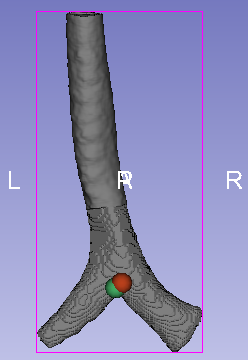
\includegraphics[height=34.5mm] {fig/Fleck_005_geometry.png}
    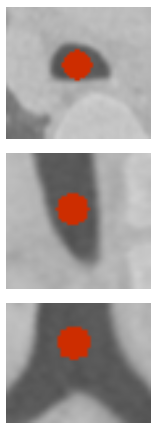
\includegraphics[height=35mm] {fig/landmark.png}
    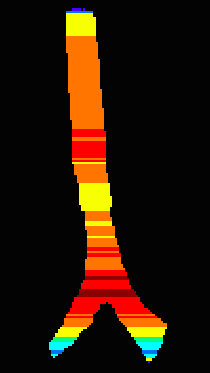
\includegraphics[height=34.5mm] {fig/Fleck_005_likelihood.png}
    \end{tabular}
    \caption{ \label{fig:detection} Visualization of the framework of landmark detection. First, an airway geometry is segmented by Otsu-thresholding. Green marker is the ground truth annotation and red marker is the predicted location of TC. Second, concatenating HOG features are computed in the center of trachea in each depth. From top to down: Sagittal, coronal, and axial. Final, applying the trained classifier on these different hypotheses to get likelihoods of the landmark. Dark red indicates the highest likelihood of TC. In this case, the predicted TC has only 1.97 mm (the total length is 159 mm) away from the ground truth annotation. The error is only 1.2$\%$.
    }
  \end{center}
\end{figure}

\section{Discussion}
\label{sec:discussion}

\bibliographystyle{splncs}
\bibliography{prp}

\end{document}
